%!TEX root = ../Thesis.tex

% 2. Theory section
% The theory used in an empirical study is meant to shed light on the data in a scholarly or scientific manner. It should give insights not achievable by ordinary, everyday reflections. The main purpose of using theory is to analyse and interpret your data. Therefore, you should not present theoretical perspectives that are not being put to use. Doing so will create false expectations, and suggests that your work is incomplete.

% Not all theses have a separate theory section. In the IMRaD format, the theory section is included in the introduction, and the second chapter covers the methods used.

% What kind of theory should you choose? Since the theory is the foundation for your data analysis it can be useful to select a theory that lets you distinguish between, and categorise different phenomena. Other theories let you develop the various nuances of a phenomenon. In other words, you have a choice of either reducing the complexity of your data or expanding upon something that initially looks simple.

% How much time and space should you devote to the theory chapter? This is a difficult question. Some theses dwell too long on theory and never get to the main point: the analysis and discussion. But it is also important to have read enough theory to know what to look for when collecting data. The nature of your research should decide: Some studies do not require much theory, but put more emphasis on the method, while other studies need a rich theory section to enable an interesting discussion.

\chapter{Theory}

\section{Calculations for differential based on steering angle} \label{diff_calc}

Due to the racing character, the vehicle was built with a parallel steering mechanism. This kind of steering is optimised accordingly to dynamics of the vehicle in high speeds. During the turn the outer wheel works under presumably higher load, therefore, having smaller slip angle than a relieved inner wheel. In a well-designed parallel steering system, these forces should cancel each other therefore we can make the calculations based on two wheels model with unchanged steering angle.\cite{vehicle_dyna}
In this model, we can simply calculate the radius of turn measuring from the rear axle by trigonometric equation \ref{diff_eq_w}.

\vspace{1em}
\begin{minipage}{0.6\textwidth}
    \begin{equation}\label{diff_eq_w}
        R = cot( \gamma ) * w
    \end{equation}
    Where:
    \begin{description}
        \item[$R$] rear axis radius (from the middle of the axis to pivot point)
        \item[$\gamma$] steering angle
        \item[$w$] wheelbase
    \end{description}
\end{minipage}
\hfill
\begin{minipage}{0.35\textwidth}
    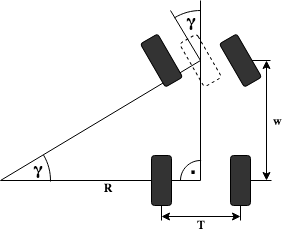
\includegraphics[width=\textwidth]{figures/diff_calc}
\end{minipage}
\vspace{1em}

Now moving back to four wheel model, since the radius is directly proportional to circumference we can calculate the proportions of how fast should wheels rotate in compare to consider rear wheel from previous model. This can be done by simply adding half of rear track to calculated radius and divide by itself.
% \begin{equation}
%     inner~wheel~proportional~speed = \frac{rear~axis~radius - rear~track / 2}{rear~axis~radius}
% \end{equation}
% \begin{equation}
%     outer~wheel~proportional~speed = \frac{rear~axis~radius + rear~track / 2}{rear~axis~radius}
% \end{equation}



\begin{equation}\label{diff_eq}
    \alpha_{inner} = \frac{R - T/2}{R}
\end{equation}
\begin{equation}
    \alpha_{outer} = \frac{R + T/2}{R} 
\end{equation}
Where:
\begin{description}
    \item[$\alpha$] wheel proportional travel
    \item[$T$] rear track
\end{description}




These numbers can be successfully used as multiplicands in the differential system for either torque or speed control loops.

\section{Regenerative Breaking} \label{regenerative_theory_section}

As explained in \cite{low_speed_regenerative_breaking} and confirmed in \cite{regen_strategy} it is not feasible to use the regenerative braking for the vehicle driving with the low speed. As the motors would generate a too small voltage to be converted up and charge the battery.
As the result the regenerative breaking should be a function of vehicle speed.

\todo{ref some research?}